\chapter{Prototype and User Study}

\section{Prototype Interface and Playback Setup}

To evaluate the generated haptic stimuli, I built a browser-based panel of stimuli that presented each visual event together with a set of anonymous vibration options. The prototype was designed as an evaluation interface rather than a real-time generation interface: all haptic stimuli were generated before the study, converted into ERM-ready playback sequences, and loaded onto the study hardware. During the study, the prototype provided a controlled way for participants to experience, replay, rate, and compare those stimuli.

\begin{figure}[!htbp]
\centering
\fbox{\parbox[c][2.2in][c]{0.88\textwidth}{\centering [TODO: insert prototype interface screenshot]}}
\caption{Prototype interface.}
\label{fig:study-prototype}
\end{figure}

For each study block, the browser displayed one fixed UI flow and a panel of anonymous haptic cards, as shown in Figure~\ref{fig:study-prototype}. Participants clicked the cards themselves to trigger individual stimuli. Selecting a card replayed the same visual flow while sending the anonymous stimulus ID to the haptic device through the Web Serial API. This design kept the visual event constant within a block, so differences in participant ratings were attributable to the haptic stimulus rather than changes in the visual presentation.

\begin{figure}[!htbp]
\centering
\fbox{\parbox[c][2.2in][c]{0.88\textwidth}{\centering [TODO: insert hardware playback diagram]}}
\caption{Hardware playback setup.}
\label{fig:hardware-playback}
\end{figure}

The hardware path was the same for every stimulus, as summarized in Figure~\ref{fig:hardware-playback}. A browser event sent the selected anonymous ID over serial to an ESP32, which selected the corresponding stored sequence and streamed it to a DRV2605L haptic driver in real-time playback mode. The driver controlled an ERM motor using the 20 ms interval drive values described in Chapter 3. Participants held the ERM motor directly between their fingers while viewing the prototype, allowing them to feel each vibration as the visual flow played.

The interface allowed flexible exploration within each flow block. Participants could experience the anonymous haptic cards in any order, replay a stimulus as many times as they wanted, and revise their ratings before moving to the next flow. After rating the individual stimuli, participants completed a block-level comparison on the same page, selecting one to three best-matching haptics and one to three worst-matching haptics and optionally explaining their choices in text. Method labels were hidden throughout the study, so participants only saw anonymous stimulus IDs rather than the generation method that produced each vibration.

\section{Study Stimuli}

The study used four controlled UI flows as representative temporal visual events: Payment Confirmation, Failed Submission, Notification Received, and Pull to Refresh. Each flow was designed as a controlled Figma prototype and then implemented in the browser panel with fixed timing, as shown in Figure~\ref{fig:study-ui-flows}. These flows were selected to cover common interaction feedback cases while placing different demands on the haptic response: success confirmation, error salience, notification arrival, and loading or progress feedback.

\begin{figure}[!htbp]
\centering
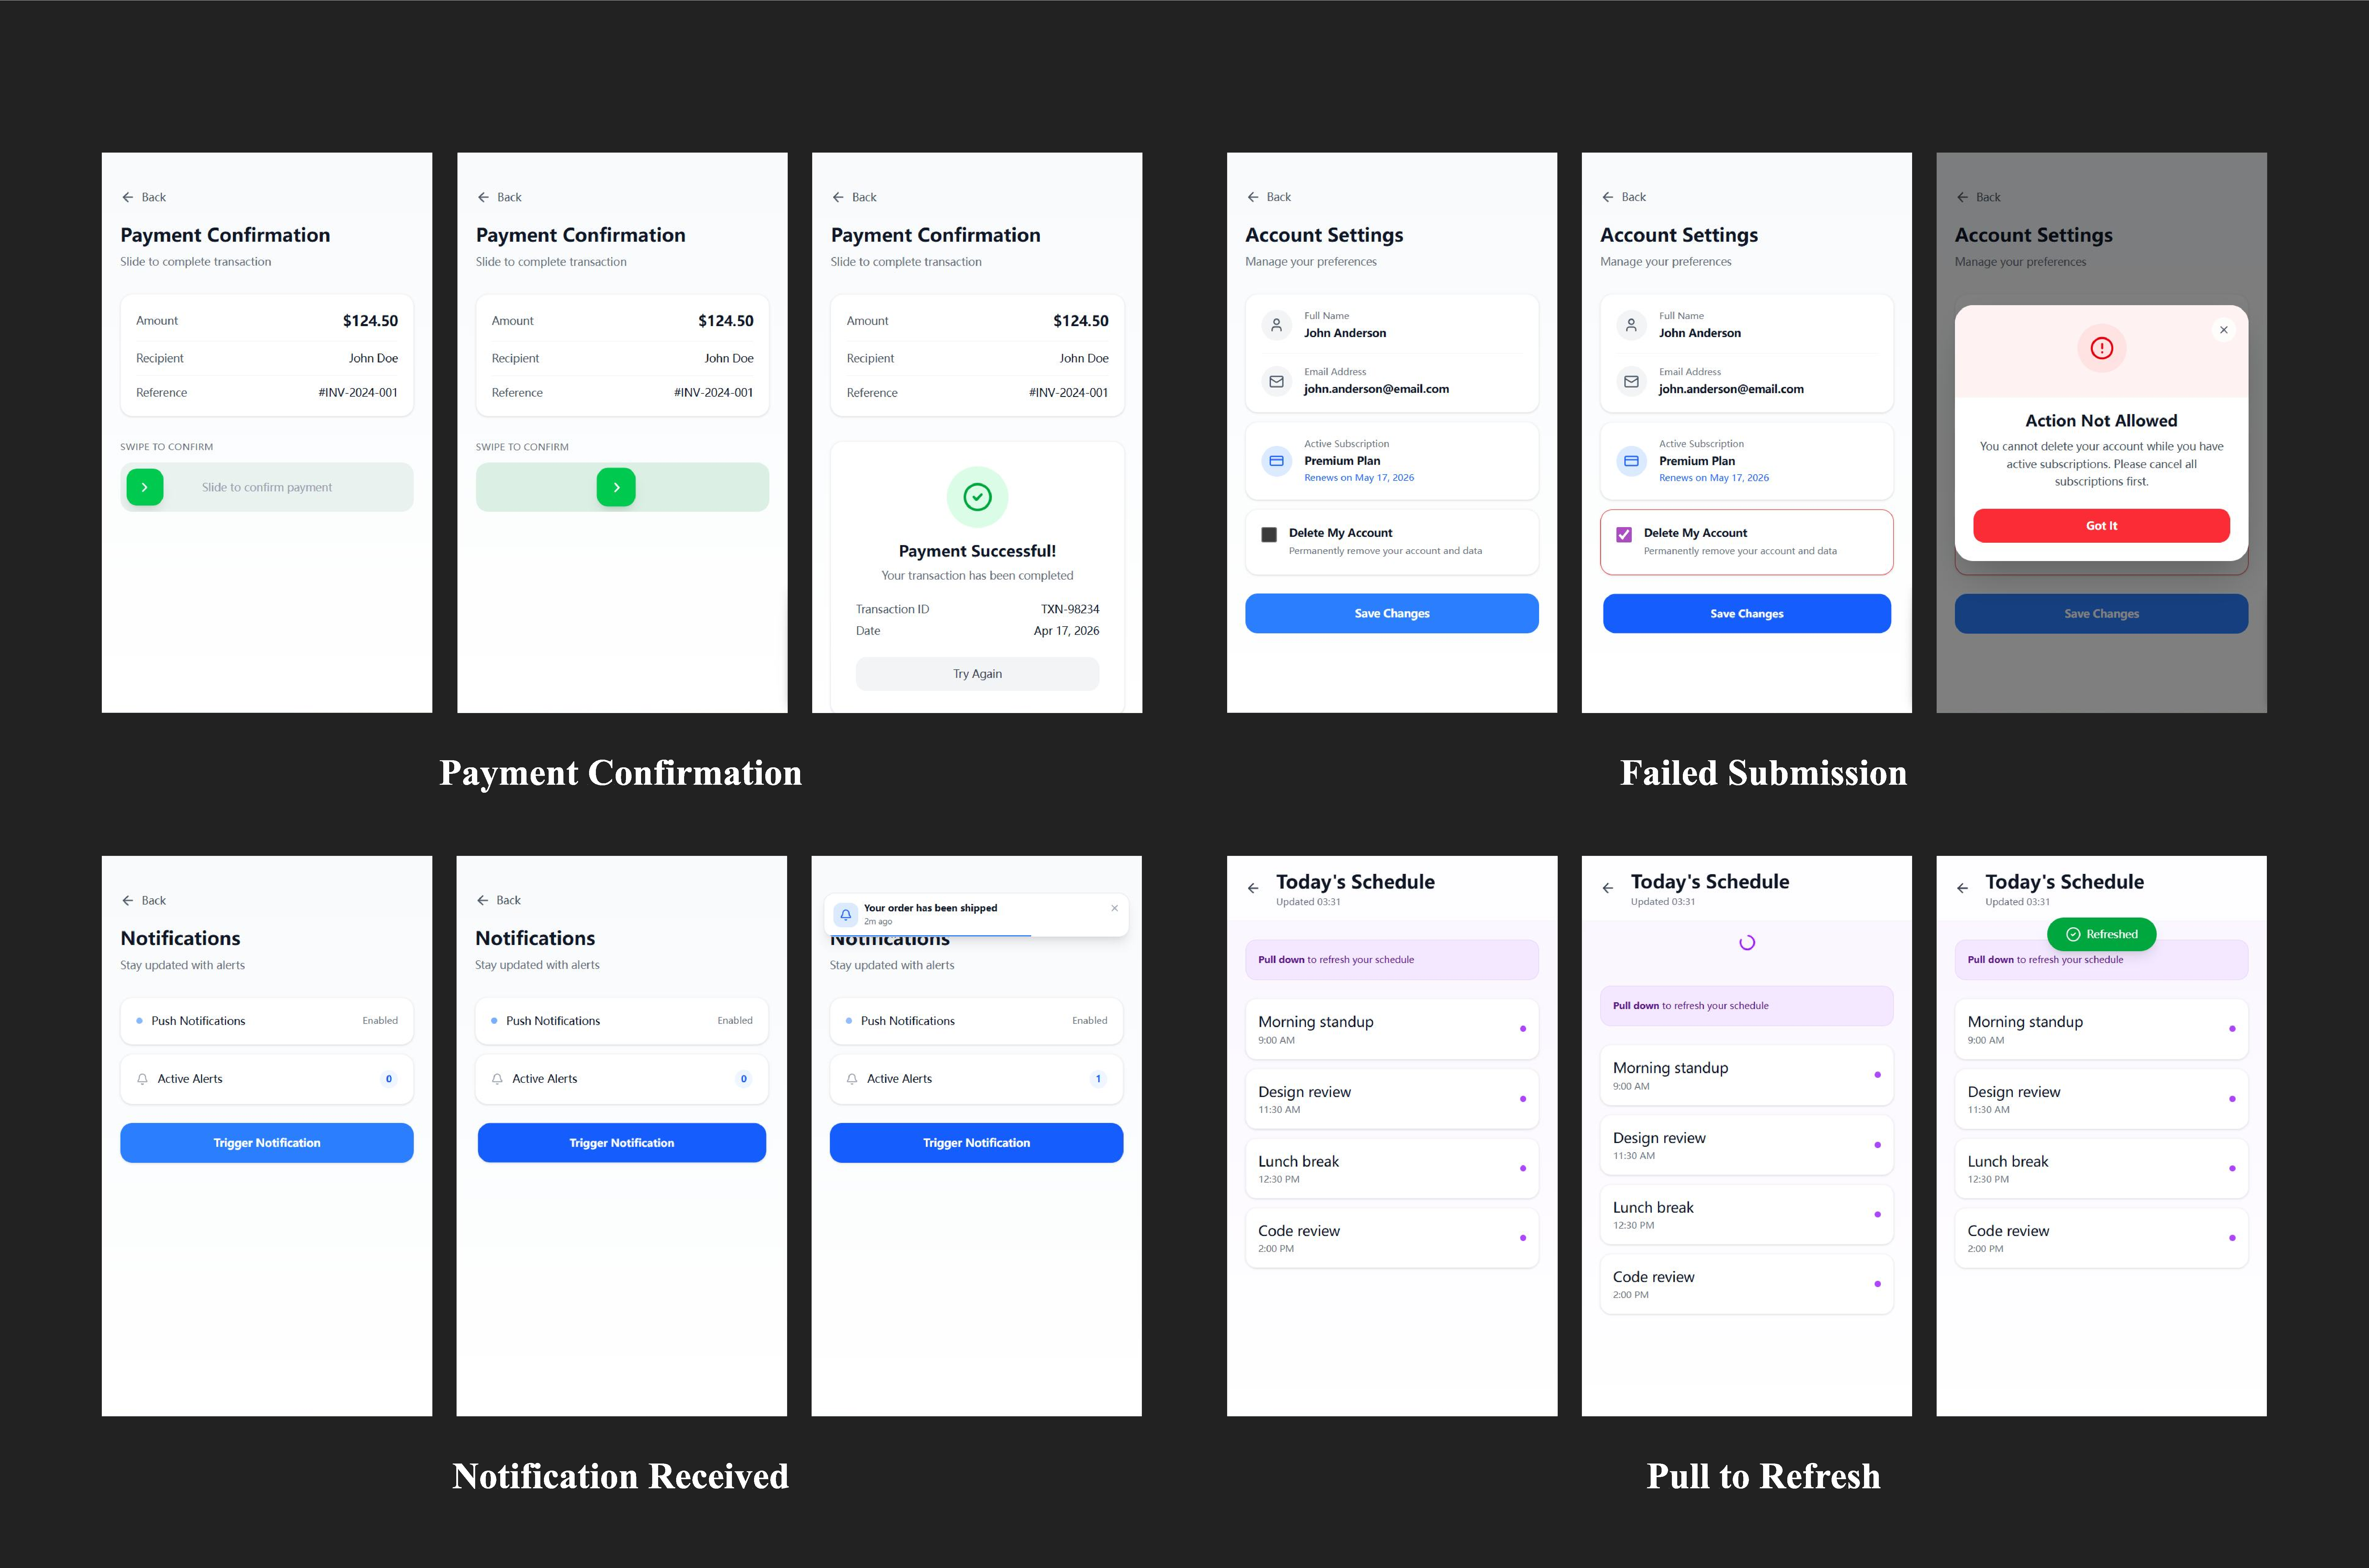
\includegraphics[width=\textwidth]{Figures/study_ui_flows.pdf}
\caption{Study UI flows.}
\label{fig:study-ui-flows}
\end{figure}

The Payment Confirmation flow shows a user sliding to confirm a payment, followed by a successful payment state. It represents a positive closure event in which haptic feedback should support a sense of completion, confidence, and confirmation. The Failed Submission flow shows a user clicking a control and receiving an error message. It represents a two-stage event in which an input action is followed by a later system refusal, making temporal separation and error salience important. The Notification Received flow shows a user pressing a trigger button and then receiving a message notification. It tests whether haptic feedback can indicate arrival or attention without feeling overly disruptive. The Pull to Refresh flow shows a downward pull gesture, a loading state, and a refreshed completion cue. It emphasizes process, motion, and completion across a longer temporal sequence.

Each flow was shown as an animated visual sequence. Within a flow block, the visual sequence was held constant while the haptic stimulus varied. This design allowed participants to compare how different vibrations fit the same temporal visual event. Each flow block contained 15 anonymous haptic stimuli, and the full study included 60 haptic stimuli across the four flows. The next section describes the generation methods represented within each set of 15 stimuli.

\section{Compared Generation Methods}

The study compared five haptic generation methods, summarized in Table~\ref{tab:generation-methods}. For each UI flow, each method contributed three variants, producing 15 anonymous stimuli per flow and 60 stimuli in total. All methods produced a two-second sequence at 10 ms intervals before being converted through the shared ERM preprocessing and playback pipeline described in Chapter 3. Except for Random Noise, the methods used the same OpenAI 4.1 model as the upstream language or vision-language component. This controlled the LLM component of the comparison while varying how its output was used for haptic generation.

\begin{table}[t]
\centering
\caption{Compared generation methods.}
\label{tab:generation-methods}
\small
\setlength{\tabcolsep}{3pt}
\renewcommand{\arraystretch}{1.15}
\begin{tabular}{@{}>{\raggedright\arraybackslash}p{1.05in}>{\raggedright\arraybackslash}p{1.6in}>{\centering\arraybackslash}p{0.6in}>{\centering\arraybackslash}p{0.9in}>{\raggedright\arraybackslash}p{1.3in}@{}}
\hline
\textbf{Method} & \textbf{Input / control signal} & \textbf{Uses VAE?} & \textbf{Uses visual event semantics?} & \textbf{Purpose in comparison} \\
\hline
Random Noise & Random 2 s sequence & $\times$ & $\times$ & Unstructured random baseline \\
Random-Plan VAE & OpenAI-generated random event plan & \checkmark & $\times$ & Structured but UI-agnostic VAE baseline \\
HapticGen & OpenAI-generated text prompt from UI images & $\times$ & \checkmark & Prompt-based generative haptic baseline \\
Direct LLM Pattern & OpenAI-authored 10 ms sequence from UI images & $\times$ & \checkmark & Direct actuator-sequence baseline \\
Semantic VAE & OpenAI-generated semantic event plan from UI images & \checkmark & \checkmark & Proposed UI-grounded semantic VAE method \\
\hline
\end{tabular}
\end{table}


Random Noise generated a fully random two-second vibration sequence. It provided the lowest-level baseline: a stimulus with no visual grounding, no semantic event structure, and no learned haptic waveform prior. This condition tested whether participants were responding to structured haptic design rather than arbitrary vibration energy.

Random-Plan VAE used the same downstream VAE generation pipeline as Semantic VAE, but its event plan was not grounded in the UI flow. The OpenAI 4.1 model was used to produce a random schema-valid haptic event plan, including behavior class, semantic role, style, strength, timing hint, duration hint, and prototype anchor. The plan was then passed through semantic target feature construction, atlas-guided latent search, VAE decoding, timeline mixing, and ERM export. This condition corresponds to the Random VAE condition in the study data, but it is more precisely described as a random-plan VAE baseline: it tests a structured but UI-agnostic version of the pipeline.

HapticGen served as a prompt-based generative haptic baseline. For each variant, the same UI flow images were first used to generate a text prompt through the OpenAI 4.1 model, and that prompt was then used as the input to HapticGen. The resulting waveform was converted to the same two-second sequence format and passed through the same ERM preprocessing pipeline as the other methods.

Direct LLM Pattern tested whether a language model could directly author a usable actuator-oriented sequence from the visual event. For each UI flow variant, the before, during, and after images were given to the OpenAI 4.1 model with instructions to output a two-second ERM-oriented sequence at 10 ms intervals. This method therefore used the visual event input but bypassed the VAE, behavior atlas, latent search, and timeline mixer.

Semantic VAE was the proposed method. It used the OpenAI 4.1 model to convert the UI flow images into a semantic haptic event plan and then generated the final stimulus through the behavior atlas, semantic-feature-guided latent search, VAE decoding, event timeline mixing, and shared ERM export. Compared with Random-Plan VAE, it tests the value of grounding the semantic event plan in the visual event. Compared with HapticGen and Direct LLM Pattern, it tests the value of separating visual-event interpretation from waveform generation through an explicit semantic intermediate representation and a learned haptic latent space.

\section{Study Procedure}

The user study used a within-subject design with 27 participants. Each participant experienced all four UI flow blocks and all five generation methods. This design allowed each participant to serve as their own comparison point across methods, reducing the effect of individual differences in haptic sensitivity and preference.

The study was organized into four flow blocks presented in a fixed order: Payment Confirmation, Failed Submission, Notification Received, and Pull to Refresh. Each block contained 15 anonymous haptic stimuli, corresponding to three variants from each of the five generation methods. Within a block, the visual flow was fixed and the anonymous card positions were randomized by a seed. Participants saw only anonymous IDs, so method labels were hidden throughout the study.

Participants completed each block at their own pace. They could click the anonymous haptic cards in any order, replay any stimulus as many times as they wanted, and revise their ratings before leaving the block. Triggering a card replayed the animated UI flow and the corresponding ERM vibration together. For each stimulus, participants gave two 7-point Likert ratings: whether the haptic clearly conveyed a meaningful response and whether it fit the visual event.

After rating the 15 stimuli in a block, participants completed a block-level comparison on the same page. They selected one to three haptics that were the best overall matches for the flow and one to three haptics that were the worst overall matches. Participants could replay stimuli while making these choices and could optionally provide text explanations for why the selected haptics were stronger or weaker fits.

Participants were allowed to pause or rest at any point. Most sessions were completed in approximately 30 minutes, while some sessions lasted up to about one hour depending on how often participants replayed stimuli and revised their responses. After completing the panel, participants filled out a follow-up survey. The survey did not collect demographic variables such as age or gender; instead, it asked about study-relevant background, including frequency of electronic-device use and how often participants notice haptic feedback in everyday devices.

\section{Measures and Analysis Plan}

The study produced three main forms of evidence: per-stimulus Likert ratings, within-flow best and worst selections, and open-text explanations. These measures were designed to capture both absolute judgments of individual stimuli and comparative preferences within the same visual event context.

For each stimulus, participants provided two 7-point Likert ratings. The first measured whether the haptic stimulus clearly conveyed a meaningful response, and the second measured whether the haptic stimulus fit the visual event. In the results analysis, ratings are summarized at the participant level for each method and flow by averaging across the three variants produced by the same method. This preserves the within-subject structure of the study and avoids treating multiple variants from the same participant and condition as independent observations. Chapter 5 reports descriptive statistics by method and flow and uses repeated-measures comparisons where appropriate, with non-parametric tests such as Friedman tests and corrected post-hoc comparisons used for method-level contrasts.

The best and worst selections provide a second measure of relative preference. Because participants selected one to three strongest and weakest matches within each flow, these responses reflect direct comparison among stimuli shown under the same visual event. Anonymous stimulus IDs are mapped back to generation methods using the stimulus key, and the analysis reports selection counts and proportions by method and flow. These counts complement the Likert ratings by showing which methods were repeatedly chosen as especially strong or especially weak matches.

Open-text explanations are analyzed using qualitative content analysis. Responses are coded with an explicit codebook covering themes such as semantic fit, timing and rhythm, intensity, smoothness, randomness, progress, comfort, and subtlety. A single response may receive multiple theme codes when it refers to more than one perceptual or semantic property. The qualitative analysis is used to interpret the rating and selection patterns rather than to replace them. The follow-up survey is used descriptively to contextualize participants' familiarity with electronic devices and everyday haptic feedback.
